\chapter{Razón Doble}
El objetivo de este capítulo es ver que, dadas dos rectas proyectivas $\proy(E)$ y $\proy(E')$, existe una homografía que transforma cuatro puntos distintos cualesquiera de $\proy(E)$ en otros cuatro puntos distintos de $\proy(E')$. Esto nos llevará a la definición de razón doble y a estudiar sus características y propiedades.

\section{Definición}
Empecemos tratando un caso más sencillo, tres puntos. Es fácil demostrar haciendo uso del álgebra lineal, como haremos a continuación, que, dadas dos rectas proyectivas, existe una única homografía que transforma tres puntos distintos cualesquiera en otros tres puntos distintos.

\begin{prop}
	\label{C5_prop_homografia3puntos}
	Dadas dos rectas proyectivas, $\proy(E)$ y $\proy(E')$, y dadas dos ternas diferentes siempre existe una única homografía que transforma la una en la otra.
\end{prop}
\begin{proof}
	Sean $\{p_0,p_1,p_2\}$ tres puntos distintos de $\proy(E)$. Al ser diferentes podemos tomar dicha terna como referencia proyectiva $\mf{R}$ de $\proy(E)$. Esto nos proporcionará una base de $E$, la correspondiente base asociada $\mc{B}$ a la referencia $\mf{R}$. Sea la terna de puntos distintos $\{p'_0,p'_1,p'_2\}$ de la recta proyectiva $\proy(E')$, podemos hacer lo mismo. Con ello obtenemos una base $\mc{B'}$ de $E'$. 
	
	Existe un único isomorfismo 
	\[\widehat{h}:E\rightarrow E'\]
	que trasforma $\mc{B}$ en $\mc{B'}$. La aplicación proyectiva asociada a esta aplicación lineal es una homografía, de hecho es biyectiva (Corolario~\ref{C4_cor_biyectividad}) que transforma $p_i$ en $p'_i$, para $i=0,1,2$. Además es única al serlo $\widehat{h}$.
\end{proof}

\begin{obs}
	La demostración de la proposición anterior nos permite deducir que dadas dos referencias proyectivas $\mf{R}$ y $\mf{R'}$ de dos rectas proyectivas, existe una única homografía que transforma $\mf{R}$ en $\mf{R'}$.
\end{obs}
Veamos un ejemplo. Para ello recordemos primero que una homografía de la recta proyectiva en sí misma, tomando la misma referencia,  puede definirse a través de coordenadas no homogéneas como
\begin{equation}
	\label{C5_eq_homografia_nohom}
	\frac{x'}{y'}=\theta'=\frac{a\frac{x}{y}+b}{c\frac{x}{y}+d}=\frac{a\theta+b}{c\theta +d}, \ \text{ tal que } ad-bc\not=0
\end{equation}
lo que denominábamos \ti{transformación de Möbius}.
\begin{exa}
	Encontrar la homografía 
	\[h:\proy^1\rightarrow \proy^1\] 
	que trasforma los puntos $\{(0:1),(1:0),(2:1)\}$ en los puntos $\{(1:1),(-1:1),(0:1)\}$.\\
	
	Podemos resolver este ejercicio de varias formas. La primera consistiría en plantear las ecuaciones con la matriz A asociada
	\begin{equation*}
		A\left( \begin{array}{c}
			x\\ y
		\end{array}\right)
		=\left( \begin{array}{cc}
			a&b\\ c&d
		\end{array}\right) 
		\left( \begin{array}{c}
			x\\ y
		\end{array}\right)=\rho
		\left( \begin{array}{c}
		x'\\ y'
	\end{array}\right)
	\end{equation*}
	y, sustituyendo los valores de los puntos dados, resolver el sistema de ecuaciones:
	\begin{equation*}
		\left( \begin{array}{cc}
			a&b\\ c&d
		\end{array}\right) 
		\left( \begin{array}{c}
			0\\ 1
		\end{array}\right)=\rho_1
		\left( \begin{array}{c}
			1\\ 1
		\end{array}\right)
	\end{equation*}
	\begin{equation*}
		\left( \begin{array}{cc}
			a&b\\ c&d
		\end{array}\right) 
		\left( \begin{array}{c}
			1\\ 0
		\end{array}\right)=\rho_2
		\left( \begin{array}{c}
			-1\\ 1
		\end{array}\right)
	\end{equation*}
	\begin{equation*}
		\left( \begin{array}{cc}
			a&b\\ c&d
		\end{array}\right) 
		\left( \begin{array}{c}
			2\\ 1
		\end{array}\right)=\rho_3
		\left( \begin{array}{c}
			0\\ 1
		\end{array}\right)
	\end{equation*}
	Sin embargo, esto puede resultar muy pesado. Si utilizamos la definición de homografía dada por la ecuación~\eqref{C5_eq_homografia_nohom}, el cálculo resulta mucho más llevadero. Así, para determinar la homografía basta hallar la expresión en coordenadas no homogéneas que la define, que se obtiene sustituyendo los valores proporcionados en la ecuación~\eqref{C5_eq_homografia_nohom} y resolviendo el sistema. Observamos que el punto $(1:0)$ se transforma en $\theta=\infty$. Para resolver esta indeterminación, se multiplica la fracción arriba y abajo por $y$
	\begin{equation}
		\theta'=\frac{a\frac{x}{y}+b}{c\frac{x}{y}+d}=\frac{ax+by}{cx +dy}
	\end{equation}
	Así, las ecuaciones resultantes son
	\begin{equation*}
		\begin{split}
			1&=\frac{a0+b1}{c0 +d1}=\frac{b}{d}\ra b=d\\
			-1&=\frac{a1+b0}{c1 +d0}=\frac{a}{c}\ra a=-c\\
			0&=\frac{a2+b1}{c2 +d1}\ra 2a+b=0
		\end{split}
	\end{equation*}
	Observamos que este sistema homogéneo es compatible indeterminado, no nos proporciona valores concretos de los coeficientes de la matriz, sino que dependen de un parámetro. En geometría proyectiva, esto es suficiente para resolver el sistema debido a que, en este caso, nos vale tanto la matriz de la aplicación lineal como un múltiplo suyo. Es decir, nos valen tanto las soluciones del sistema como un múltiplo suyo, \tb{rayos de soluciones}.
	
	Así, para el caso que nos ocupa, $a=\lambda$ y con ello $c=-\lambda, \ b=-2\lambda$ y $d=-2\lambda$, siendo así la matriz
	\begin{equation*}
	 \lambda \left( \begin{array}{cc}
	 1&-2\\ -1&-2
	 \end{array}\right) 
	\end{equation*}
	y podemos tomar sin ningún problema $\lambda=-1$.
	
	Por lo que, tomando $a=-1$, la homografía pedida viene dada por
	\begin{equation*}
		\theta'=\frac{2-\theta}{2+\theta}
	\end{equation*}
	Nótese que no es necesario tener tanto cuidado con $\theta=\infty$, como ya se explicó en el capítulo anterior. Si tenemos en cuenta que $\infty+b=\infty$ y que $\frac{\infty}{\infty}=1$, el resultado es el mismo
	\begin{equation*}
		\theta'=-1=\frac{a\theta+b}{c\theta +d}=\frac{a\infty+b}{c\infty +d}=\frac{a\infty}{c\infty}=\frac{a}{c}\ra a=-c
	\end{equation*}
\end{exa}
\begin{obs}
	De lo explicado en el ejemplo anterior acerca de los sistemas que se obtienen al trabajar con coordenadas no homogéneas se deduce que, para determinar una homografía de $\proy^1$, son suficientes $3$ puntos y sus imágenes, pues nos vale con obtener un rayo de soluciones.
\end{obs}
Encontrar una homografía de una recta proyectiva que lleve cuatro puntos distintos cualesquiera en otros cuatro no es tan sencillo. Para poder caracterizar esta propiedad empezaremos estudiando las características de una homografía que la cumpla.
\begin{lem}
	Sean $\{p_1,p_2,p_3,p_4\}$ y $\{p'_1,p'_2,p'_3,p'_4\}$ ocho puntos distintos de la recta proyectiva $\proy(E)$ respecto a la referencia $\mf{R}$. Sea una homografía
	\[h:\proy(E)\rightarrow \proy(E)\]
	que cumple $h(\theta_i)=\theta'_i$ para todo $i\in\{1,2,3,4\}$, donde $\theta_i$ es el parámetro no homogéneo de $p_i$. Entonces
	\begin{equation}
		\frac{\theta_3-\theta_1}{\theta_3-\theta_2}:\frac{\theta_4-\theta_1}{\theta_4-\theta_2}=\frac{\theta'_3-\theta'_1}{\theta'_3-\theta'_2}:\frac{\theta'_4-\theta'_1}{\theta'_4-\theta'_2}
	\end{equation}
\end{lem}
\begin{proof}
	Dado que $h$ es una homografía de una recta proyectiva en sí misma, y hemos tomado la misma referencia, podemos escribir
	\begin{equation*}
		\theta'=\frac{a\theta+b}{c\theta +d}\tq ad-bc\not=0
	\end{equation*}
	para determinados $a,b,c$ y $d$. Así
	\begin{equation*}
		\frac{\theta'_3-\theta'_1}{\theta'_3-\theta'_2}:\frac{\theta'_4-\theta'_1}{\theta'_4-\theta'_2}=\frac{\frac{a\theta_3+b}{c\theta_3 +d}-\frac{a\theta_1+b}{c\theta_1 +d}}{\frac{a\theta_3+b}{c\theta_3 +d}-\frac{a\theta_2+b}{c\theta_2 +d}}:\frac{\frac{a\theta_4+b}{c\theta_4 +d}-\frac{a\theta_1+b}{c\theta_1 +d}}{\frac{a\theta_4+b}{c\theta_4 +d}-\frac{a\theta_2+b}{c\theta_2+d}}
	\end{equation*}
	Operando se obtiene
	\begin{equation*}
		\frac{\theta'_3-\theta'_1}{\theta'_3-\theta'_2}:\frac{\theta'_4-\theta'_1}{\theta'_4-\theta'_2}=\frac{\frac{(\theta_3-\theta_1)(ad-bc)}{(c\theta_3+d)(c\theta_1+d)}}{\frac{(\theta_3-\theta_2)(ad-bc)}{(c\theta_3+d)(c\theta_2+d)}}:\frac{\frac{(\theta_4-\theta_1)(ad-bc)}{(c\theta_4+d)(c\theta_1+d)}}{\frac{(\theta_4-\theta_2)(ad-bc)}{(c\theta_4+d)(c\theta_2+d)}}=\frac{\theta_3-\theta_1}{\theta_3-\theta_2}:\frac{\theta_4-\theta_1}{\theta_4-\theta_2}
	\end{equation*}
\end{proof}
Por tanto, toda homografía de una recta proyectiva en sí misma que lleve cuatro puntos distintos a otros cuatro, mantiene invariante el cociente 
\begin{equation*}
	\frac{\theta_3-\theta_1}{\theta_3-\theta_2}:\frac{\theta_4-\theta_1}{\theta_4-\theta_2}
\end{equation*}
Conviene entonces dar un nombre a dicho cociente.
\begin{defi}[Razón doble]
	Sean cuatro puntos diferentes de una recta proyectiva $\{p_1,p_2,p_3,p_4\}$, se define su \ti{razón doble} como el cociente
	\begin{equation}
	\{p_1,p_2;p_3,p_4\}=\{\theta_1,\theta_2;\theta_3,\theta_4\}=\frac{\theta_3-\theta_1}{\theta_3-\theta_2}:\frac{\theta_4-\theta_1}{\theta_4-\theta_2}
	\end{equation}
	donde $\theta_i$ es el parámetro no homogéneo de $p_i$ respecto a una referencia $\mf{R}$ de la recta proyectiva.
\end{defi}
\begin{obs}
	Dado que $\theta_i$ es el parámetro no homogéneo de $p_i$, el cálculo de la razón doble se puede hacer también usando coordenadas homogéneas. Si $p_i=(x_i,y_i)$, entonces, sustituyendo en la definición y operando
	\begin{equation*}
		\{p_1,p_2;p_3,p_4\}=\frac{\frac{x_3}{y_3}-\frac{x_1}{y_1}}{\frac{x_3}{y_3}-\frac{x_2}{y_2}}:\frac{\frac{x_4}{y_4}-\frac{x_1}{y_1}}{\frac{x_4}{y_4}-\frac{x_2}{y_2}}=\frac{(x_3y_1-x_1y_3)/y_1y_3}{(x_3y_2-x_2y_3)/y_3y_2}:\frac{(x_4y_1-x_1y_4)/y_4y_1}{(x_4y_2-x_2y_4)/y_4y_2}
	\end{equation*}
	la razón doble se puede escribir como
	\begin{equation}
	\{p_1,p_2;p_3,p_4\}=\frac{
		\left| \begin{array}{cc}
				x_3&x_1\\
				y_3&y_1
		\end{array}\right|}{
		\left| \begin{array}{cc}
		x_3&x_2\\
		y_3&y_2
		\end{array}\right|}:\frac{
		\left| \begin{array}{cc}
		x_4&x_1\\
		y_4&y_1
		\end{array}\right|}{
		\left| \begin{array}{cc}
		x_4&x_2\\
		y_4&y_2
		\end{array}\right|}
	\end{equation}
	Observemos que, como los puntos son distintos las columnas de los determinantes no son proporcionales y, por tanto, ningún determinante es nulo.
\end{obs}
Con esta definición el lema se traduce en que toda homografía de una recta proyectiva en sí misma, que lleve cuatro puntos diferentes cualesquiera en otros cuatro, mantiene invariante la razón doble. Consecuencia de este resultado es el corolario siguiente.
\begin{cor}
	Dada una homografía $h$ de la recta en sí misma y dados cuatro puntos distintos cualesquiera $\{p_1,p_2,p_3,p_4\}$, se cumple que $h$ preserva la razón doble:
	\begin{equation}
	\{p_1,p_2;p_3,p_4\}=\{h(p_1),h(p_2);h(p_3),h(p_4)\}
	\end{equation} 
\end{cor}
\begin{proof}
	Dado que $\{p_1,p_2,p_3,p_4\}$ son distintos y una homografía es una aplicación proyectiva inyectiva, los puntos $\{h(p_1),h(p_2),h(p_3),h(p_4)\}$ son distintos.
	
	Por otro lado, denotando $p_i=(x_i:y_i)$ y $h(p_i)=(x'_i:y'_i)$ y teniendo en cuenta que toda homografía se puede describir con la relación
	\begin{equation*}
		\theta'=\frac{a\theta+b}{c\theta +d}
	\end{equation*}
	para determinados $a,b,c$ y $d$, donde $\theta=\frac{x_i}{y_i}$ y $\theta'=\frac{x'_i}{y'_i}$, es obvio que $h(\theta_i)=h(\frac{x_i}{y_i})=\frac{x'_i}{y'_i}=\theta'_i$ para todo $i\in\{1,2,3,4\}$. Del lema anterior se deduce que
	\begin{equation*}
		\{p_1,p_2;p_3,p_4\}=\{h(p_1),h(p_2);h(p_3),h(p_4)\}
	\end{equation*}
\end{proof}
\begin{obs}
	Observamos que la razón doble está bien definida, es decir, que no depende de la referencia elegida. En efecto, sean cuatro puntos distintos $x_1,x_2,x_3,x_4$ en la referencia $\mf{R}$. Dada otra referencia $\mf{R}'$, las coordenadas de dichos puntos en esta nueva referencia serán $x_1'=Px_1,x_2'=Px_2,x_3'=Px_3,x_4'=Px_4$, siendo $P$ una matriz de paso. Cada uno de estos puntos podemos verlo como la imagen de una aplicación proyectiva definida por la matriz $P$, es decir, $Px_i=h(x_i)$. Como $P$ es invertible, $h$ es una homografía. El corolario anterior nos asegura entonces que la razón doble de $x_1,x_2,x_3,x_4$ es la misma que la de $x'_1,x'_2,x'_3,x'_4$.
\end{obs}
Hasta ahora hemos establecido varias relaciones entre las homografías y la razón doble. Hemos visto que no solo las homografías de una recta proyectiva en sí misma que transforma cuatro puntos distintos cualesquiera en otros cuatro conserva la razón doble, sino todas las homografías de una recta proyectiva en sí misma. El recíproco de ambos también es cierto. Sin embargo, en vez de demostrarlo para este caso particular, generalicemos lo resultados a homografías de una recta proyectiva $\proy(E)$ a otra recta $\proy(E')$.

\section{Propiedades}
La razón doble ha sido descrita respecto a una referencia $\mf{R}$ arbitraria de la recta proyectiva, por lo que esta puede ser calculada respecto a cualquier referencia. Si dados cuatro puntos distintos $\{p_1,p_2,p_3,p_4\}$ de $\proy(E)$ tomamos como referencia de la recta $\mf{R}=\{p_1,p_2,p_3\}$, lo cual es posible al ser diferentes, entonces las coordenadas homogéneas de los cuatro puntos pasan a ser
\begin{equation*}
	\{(1:0),(0:1),(1:1),(\alpha:\beta)\}
\end{equation*}
donde $(\alpha:\beta)$ son las coordenadas homogéneas de $p_4$ respecto a la referencia. Si calculamos la razón doble obtendríamos que 
\begin{equation}
	\{p_1,p_2;p_3,p_4\}=\{(1:0),(0:1);(1:1),(\alpha:\beta)\}=\{\infty,0;1,\frac{\alpha}{\beta}\}=\frac{\alpha}{\beta}
\end{equation}
Surge así una nueva definición de razón doble.
\begin{defi}(Razón doble)
	La razón doble de cuatro puntos distintos de una recta proyectiva es la coordenada no homogénea del cuarto punto respecto a la referencia formada por los tres primeros.
\end{defi}
Una vez dada esta definición podemos generalizar los resultados obtenidos en el apartado anterior. Para ello hagamos antes una pequeña observación.
\begin{obs}
	\label{C5_obs_coordenadas_p_g(p)}
	Sea $g:\proy(E)\rightarrow \proy(E')$ la única homografía que trasforma $\mf{R}=\{a,b,c\}$ en $\mf{R'}=\{a',b',c'\}$. Sea un punto $p\in \proy(E)$ cuyas coordenadas respecto a la referencia $\mf{R}$ son $p=(\alpha:\beta)_{\mf{R}}$. Indicaremos un vector representante de un punto $q$ por $\vec{q}$. Entonces, teniendo en cuenta que $\widehat{g}$ es lineal, se tiene que 
	\begin{equation*}
		g(p)=\class{\widehat{g}(\vec{p})}=\class{\widehat{g}(\alpha \vec{a}+\beta \vec{b})}=\class{\alpha \widehat{g}( \vec{a})+\beta \widehat{g}(\vec{b})}=\class{\alpha \vec{a}'+\beta \vec{b}'}=(\alpha:\beta)_{\mf{R}'}
	\end{equation*}
	Por tanto, las coordenadas de $p$ respecto a la referencia $\mf{R}$ son las mismas que las coordenadas de $g(p)$ respecto a $\mf{R'}$.
\end{obs}
\begin{theo}\label{C5_teo_hom4puntos_sii_razondoble}
	Sean $\proy(E)$ y $\proy(E')$ dos rectas proyectivas, $a,b,c,d$ puntos distintos de $\proy(E)$ y $a',b',c',d'$ puntos distintos de $\proy(E')$. Entonces, existe una homografía $h:\proy(E)\rightarrow \proy(E')$ que transforma los puntos $a,b,c,d$ en los puntos $a',b',c',d'$ respectivamente si y solo si 
	\begin{equation*}
		\{a,b;c,d\}=\{a',b';c',d'\}
	\end{equation*}
\end{theo}
\begin{proof} Tomamos como referencia de $\proy(E)$ los puntos $\mf{R}=\{a,b,c\}$ y como referencia de $\proy(E')$ los puntos $\mf{R}'=\{a',b',c'\}$. Sean $\rho(d)$ las coordenadas de $d$ respecto a $\mf{R}$ y $\rho'(d')$ las coordenadas de $d'$ respecto a $\mf{R}'$. Por la definición anterior de razón doble sabemos que 
\begin{equation*}
	\{a,b;c,d\}=\rho(d) \qquad y \qquad \{a',b';c',d'\}=\rho'(d')
\end{equation*}
Sea $g:\proy(E)\rightarrow \proy(E')$ la única homografía que trasforma $\mf{R}$ en $\mf{R'}$. Entonces, por la observación~\ref{C5_obs_coordenadas_p_g(p)}, las coordenadas de $d$ respecto a $\mf{R}$ son las mismas que las coordenadas de $g(d)$ respecto a $\mf{R'}$. Siguiendo nuestra notación $\rho(d)=\rho'(g(d))$.\\

\bra \ Supongamos que existe una homografía $h:\proy(E)\rightarrow \proy(E')$ que transforma los puntos $a,b,c,d$ en los puntos $a',b',c',d'$ respectivamente. Entonces $\rho'(d')=\rho'(h(d))$. Dado que $g$ es única y $h$ transforma $a$ en $a'$, $b$ en $b'$ y $c$ en $c'$, es decir $\mf{R}$ en $\mf{R'}$, se tiene que $h=g$. Con ello \\
$\rho'(d')=\rho'(h(d))=\rho'(g(d))=\rho(d)$, dándose así la igualdad de razones dobles.\\

\bla \ Supongamos que se da la igualdad de razones dobles. Entonces $\rho'(d')=\rho(d)=\rho'(g(d))$. Por tanto, las coordenadas de $d'$ respecto a $\mf{R}'$ son las mismas que las coordenadas de $g(d)$ respecto a la misma referencia. Esto implica que $g(d)=d'$, con lo que $g$ es la homografía $h$ que buscábamos.
\end{proof}
Observemos que en la demostración hemos concluido que $h=g$. Esto nos permite reenunciar el teorema de la siguiente forma.\\

\tb{Teorema 5.2.1} Sea $h:\proy(E)\rightarrow \proy(E')$ la única  homografía que transforma $a,b,c$ en $a',b',c'$. Entonces 
\begin{equation}
		h(d)=d' \sii \{a,b;c,d\}=\{a',b';c',d'\}.
\end{equation}
\begin{cor}
	Las homografías de rectas proyectivas son las biyecciones que conservan la razón doble.
\end{cor}
\begin{proof}
	Demostremos primero que dada una homografía de rectas proyectivas, esta preserva la razón doble. 
	
	Sea $h:\proy(E)\rightarrow \proy(E')$ una homografía de rectas proyectivas y denotemos $h(a)=a'$, $h(b)=b'$, $h(c)=c'$. Es obvio que acabamos de construir la única homografía que transforma $a,b,c$ en $a',b',c'$. Tomando $d'=h(d)$, por el teorema anterior, se tiene que $\{a,b;c,d\}=\{a',b';c',d'\}$.\\
	
	Demostremos el recíproco. Dada $g:\proy(E)\rightarrow \proy(E')$ biyección que conserva la razón doble, denotamos $g(a)=a'$, $g(b)=b'$, $g(c)=c'$. Sea, por otro lado, $h:\proy(E)\rightarrow \proy(E')$ la única homografía de rectas que transforma $a,b,c$ en $a',b',c'$. Como $g$ conserva la razón doble, si denotamos $g(d)=d'$ se tiene que $\{a,b;c,d\}= \{g(a),g(b),g(c),g(d)\}=\{a',b';c',d'\}$. Por tanto, aplicando el teorema anterior esto implica que $h(d)=d'=g(d)$. Como $d$ es arbitrario, se tiene que $h=g$, con lo cual $g$ es homografía de rectas.
\end{proof}
Como se puede observar en la demostración, la razón doble nos permite definir homografías. Veamos un ejemplo para que esto quede claro.
\begin{exa}
	Encontrar una homografía $h:\proy^1\rightarrow \proy^1$ tal que 
	\begin{equation*}
		\begin{array}{cccc}
		h:&0&\rightarrow &\infty\\
		&1&\rightarrow &-1\\
		&-1&\rightarrow &0
		\end{array}
	\end{equation*}
	Se tiene que $h$ es la única homografía que lleva el $0$ al $\infty$, el $1$ al $-1$ y el $-1$ al $0$. Nótese que se puede enunciar el teorema anterior con las coordenadas no homogéneas de los puntos sin problema alguno. Por tanto, podemos aplicar el corolario, según el cual $h$, al ser una homografía de rectas proyectivas, conserva la razón doble, es decir
	\begin{equation*}
		\{0,1;-1,\theta\}=\{h(0),h(1);h(-1),h(\theta)=\theta'\}=\{\infty,-1;0;\theta'\}
	\end{equation*}
	Desarrollando las razones dobles
	\begin{equation*}
		\frac{0+1}{0-\theta}:\frac{0-\theta}{1-\theta}=\frac{\infty-0}{-1-0}:\frac{\infty-\theta'}{-1-\theta'}
	\end{equation*}
	Dado que $h$ es una homografía de $\proy^1$ en $\proy^1$, basta encontrar la transformación de möbius para describirla por completo, es decir, la relación entre $\theta$ y $\theta'$. Para ello operamos y despejamos, obteniendo
	\begin{equation*}
		\theta'=\frac{-\theta-1}{2\theta}
	\end{equation*}
	Por tanto, la homografía $h$ tal que $\theta'=\frac{-\theta-1}{2\theta}$ es la homografía pedida.
\end{exa}

\section{Simetrías de la razón doble}\label{C5_sec_simetrias}

La razón doble ha sido descrita como un cociente de parámetros no homogéneos ordenados de la siguiente manera $\{\theta_1,\theta_2;\theta_3,\theta_4\}$. Cabe preguntarse si las 24 posibles permutaciones de las coordenadas $\theta_i$ darán la misma razón doble.

A continuación se dará el valor de la razón doble resultante de permutar las coordenadas no homogéneas, respecto a $\{\theta_1,\theta_2;\theta_3,\theta_4\}$. Dado que para probar dichos resultados basta con aplicar la definición de razón doble, desarrollar el cociente y simplificar, las comprobaciones se dejan al lector. 

Dada la razón doble $\{\theta_1,\theta_2;\theta_3,\theta_4\}$, se tiene que:
\begin{itemize}
	\item Permutar la primera y la segunda componente por un lado, y la tercera y la cuarta por otro, mantiene invariante la razón doble: \[\{\theta_1,\theta_2;\theta_3,\theta_4\}=\{\theta_2,\theta_1;\theta_4,\theta_3\}\]
	
	\item Permutar el par $\theta_1,\theta_2$ con el par $\theta_3,\theta_4$, mantiene invariante la razón doble: \[\{\theta_1,\theta_2;\theta_3,\theta_4\}=\{\theta_3,\theta_4;\theta_1,\theta_2\}\]
	
	\item Si $\{\theta_1,\theta_2;\theta_3,\theta_4\}=\lambda$, entonces:
	\begin{equation*}
		\begin{split}
			\{\theta_1,\theta_3;\theta_2,\theta_4\}&=1-\lambda\\
			\{\theta_2,\theta_1;\theta_3,\theta_4\}&=\frac{1}{\lambda}\\
			\{\theta_2,\theta_3;\theta_1,\theta_4\}&=1-\frac{1}{\lambda}\\
			\{\theta_3,\theta_1;\theta_2,\theta_4\}&=\frac{1}{1-\lambda}\\
			\{\theta_3,\theta_2;\theta_1,\theta_4\}&=\frac{\lambda}{1-\lambda}
		\end{split}
	\end{equation*}
\end{itemize}
Esto nos da las 24 reordenaciones posibles. Resulta entonces que si $\{\theta_1,\theta_2;\theta_3,\theta_4\}=\lambda$, los valores que aparecen al efectuar todas las permutaciones son 
\[\lambda,1-\lambda,\frac{1}{\lambda},1-\frac{1}{\lambda},\frac{1}{1-\lambda},\frac{\lambda}{1-\lambda}\]
\section{Cuaternas Armónicas}
\begin{defi}[Cuaterna armónica]
	Diremos que $p_1,p_2,p_3,p_4$ es una \ti{cuaterna armónica}, o que el par $p_1,p_2$ separa armónicamente al par $p_3,p_4$, si su razón doble es $-1$.
	\begin{equation}
		\{p_1,p_2;p_3,p_4\}=-1
	\end{equation}
\end{defi}
Si cuatro puntos de una recta proyectiva son una cuaterna armónica, entonces es posible hacer la siguiente construcción geométrica, denominada \tb{cuadrilátero completo}, donde $p_1D$, $p_2D$ y $p_1F$ son rectas arbitrarias, por tanto también lo son los puntos $D$ y $F$.

\begin{figure}[h]
	\centering
	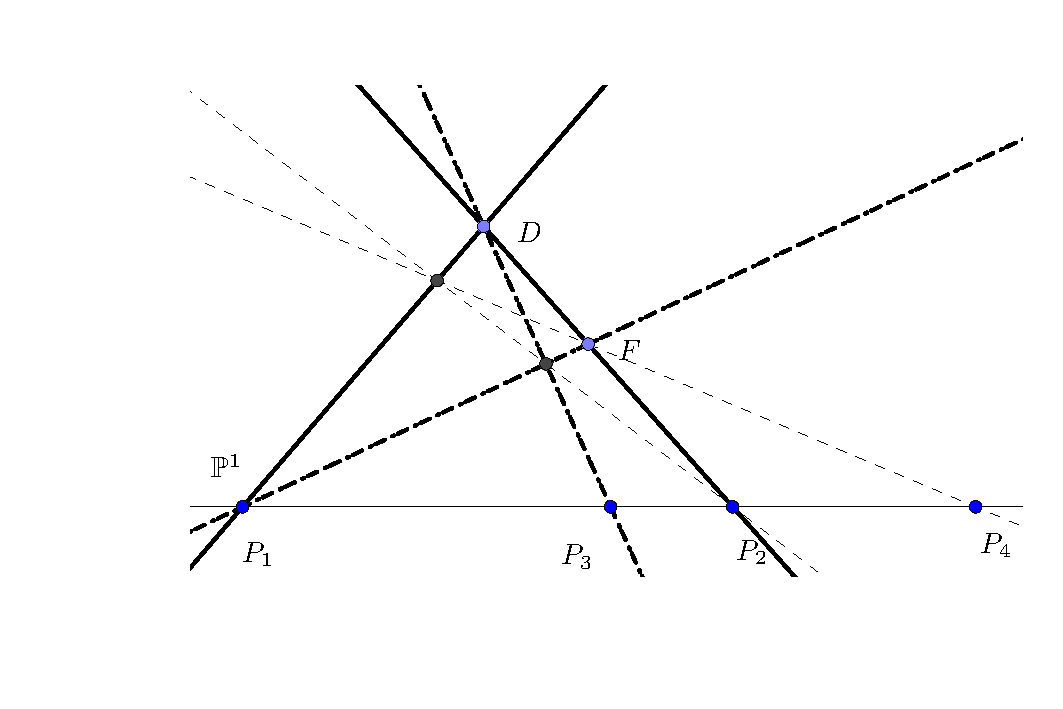
\includegraphics[scale=.6]{Graficos/RazonDoble/razon_doble}
	\caption{Cuaterna armónica}
	\label{C5_img_cuaterna_armonica}
\end{figure}

El recíproco también es cierto, como se muestra en la siguiente proposición.
\begin{prop}
	Dado el cuadrilátero completo formado por los puntos $p_1,p_2,p_3$ y $p_4$, construcción geométrica mostrada en la figura~\ref{C5_img_cuaterna_armonica}, se tiene que $\{p_1,p_2;p_3,p_4\}=-1$.
	
\end{prop}
\begin{proof}
	Tomamos como referencia los puntos $p_1,p_2,p_{arbitario}$ y el punto de corte de las rectas $p_1F$ y $p_3D$, que denotaremos $e$. Esto es posible ya que, como se observa en la figura, son proyectivamente independientes.
	\[\mf{R}=\{p_1,p_2,D;e\}\]
	Debemos entonces expresar los puntos $p_1,p_2,p_3$ y $p_4$ respecto a esta referencia. Los primeros son sencillos, $p_1=(1:0:0)$ y $p_2=(0:1:0)$. 
	
	Por otro lado, $p_3$ es la intersección de las rectas $ep_{arbitario}$ y $p_1p_2$. Estas pueden ser descritas por las ecuaciones
	\begin{equation*}
		eD:=\class{\alpha(1,1,1)+\beta(0,0,1)\tq \alpha,\beta\in \R}=(1:1:1+\theta)\cup\{D\}\tq\theta\in\R
	\end{equation*}
	\begin{equation*}
		p_1p_2:z=0
	\end{equation*}
	siendo por tanto el punto de corte 
	\[p_3=(1:1:0)\]
	De la misma forma podemos calcular $p_4$ como la intersección de las rectas $p_1p_2$ y $DF$, donde $D$ es el punto de corte de las rectas $p_1D$ y $p_2e$. Por tanto, para calcular las coordenadas de $p_4$ respecto a la referencia $\mf{R}$, primero debemos obtener las de $D$ y las de $F$.
	
	Comencemos con $D$. Las rectas de las cuales es intersección pueden describirse a través de 
	\begin{equation*}
		p_2e:\class{\alpha(1,1,1)+\beta(0,1,0)\tq\alpha,\beta\in \R}=(1:1+\theta:1)\cup\{p_2\}\tq\theta\in\R
	\end{equation*}
	\begin{equation*}
		p_1D:y=0
	\end{equation*}
	por lo que el punto buscado es
	\[D=(1:0:1)\]
	Para calcular $F$ tenemos que las rectas correspondientes vienen dadas por
	\begin{equation*}
		p_1F:\class{\alpha(1,1,1)+\beta(1,0,0)\tq\alpha,\beta\in \R}=(1+\theta:1:1)\cup\{p_1\}\tq\theta\in\R
	\end{equation*}
	\begin{equation*}
		p_2D:x=0
	\end{equation*}
	siendo el punto de corte
	\[F=(0:1:1)\]
	Podemos ya calcular las coordenadas de $p_4$ como la intersección de 
	\begin{equation*}
		DF:\class{\alpha(1,0,1)+\beta(0,1,1)\tq\alpha,\beta\in \R}=(1:\theta:1+\theta)\cup\{F\}\tq\theta\in\R
	\end{equation*}
	\begin{equation*}
		p_1p_2:z=0
	\end{equation*}
	Con ello obtenemos que
	\[p_4=(1:-1:0)\]
	Una vez hecho esto basta comprobar que la razón doble de $p_1,p_2p_3$ y $p_4$ es $-1$. Para ello haremos uso de resultados del apartado de cálculo de razones dobles, ya que de momento no hemos visto cómo calcular la razón doble de puntos que no pertenecen a una recta proyectiva, como es el caso.
	
	Entonces, como veremos más adelante
	\begin{equation}
		\{p_1,p_2;p_3,p_4\}=\{(1:0:0),(0:1:0);(1:1:0),(1:-1:0)\}=\{\infty,0;1,-1\}=-1
	\end{equation}
\end{proof}
dado que en esta construcción las rectas $p_1D$, $p_2D$ y $p_1F$ y los puntos $D$ y $F$ son arbitrarios, elijamos los que elijamos vamos a obtener siempre el mismo punto $p_4$. 

El orden de la cuaterna armónica es relativamente importante ya que, aunque algunas permutaciones cambian su valor, las reordenaciones
\begin{equation*}
	\{p_2,p_1;p_4,p_3\}, \quad \{p_3,p_4;p_1,p_2\}, \quad \{p_2,p_1;p_3,p_4\}
\end{equation*}
siguen dando como resultado $-1$.

Es importante mencionar varias cosas acerca de esta construcción. El punto $p_3$ está entre el punto $p_1$ y el punto medio entre $p_1$ y $p_2$ si y solo si el punto $p_4$ está a la izquierda de $p_1$. Por el contrario, $p_3$ está entre el punto medio y el punto $p_2$  si y solo si el punto $p_4$ está a la derecha de $p_2$. Si el punto $p_3$ no está entre $p_1$ y $p_2$, entonces lo estará $p_4$. Por último, $p_3$ está en el punto medio si y solo si $p_4$ está en el infinito. Esto significa que la recta $p_4F$ es paralela a la recta donde se encuentran los puntos.

Observemos que si, al calcular la razón doble tomamos como referencia los puntos $p_1,p_2,p_3$, entonces, necesariamente, $\theta_4=-1$.
\begin{equation*}
	\{p_1,p_2;p_3,p_4\}=\{\infty,0,1,-1\}=-1
\end{equation*}

\section{Cálculo de la Razón Doble en $\proy^n$}
\label{C5_generalizacionesRazonDoble}
Hasta ahora, sólo hemos calculado la razón doble de cuatro puntos de $\proy^1$. Sin embargo, será útil con frecuencia calcular la razón doble de cuatro puntos alineados en un espacio proyectivo de dimensión finita arbitraria.
 
En esta sección, trataremos de ofrecer procedimientos para realizar estos cálculos de forma eficiente.

Además, para rizar el rizo, y sin salir demasiado de nuestro propósito original, estudiaremos algunas de las relaciones de la razón doble con la dualidad.
\subsection{Razón Doble en $\proy^n$}
En este apartado trataremos de generalizar la noción de razón doble para cuatro puntos alineados de $\proy^n$. Para ello, daremos dos procedimientos distintos que es útil saber dominar. Ambos serán ilustrados con ejemplos (que se recomienda no omitir) para que calen mejor en el lector.
\subsubsection{Procedimiento Referencial}
Sean una recta $r$ de $\proy^n$ y cuatro puntos proyectivos $A,B,C,D\in r$. Para calcular la razón doble de dichos cuatro puntos, tomemos una referencia ``cómoda'' de la recta $r$. De esta forma, los puntos quedan expresados con dos coordenadas homogéneas, pudiendo aplicar los procedimientos de cálculo habituales. Veámoslo con un ejemplo.
\begin{exa}[Cuatro Puntos Alineados]
	\label{C5_exa_puntosAlineados}
	Sean los puntos alineados (compruébese):
	\[\begin{array}{c}
	A=(1:0:-1)=\class{\vec{a}}\\
	B=(2:1:0)=\class{\vec{b}}\\
	C=(4:1:-2)=\class{2\vec{a}+\vec{b}}\\
	D=(-1:-1:-1)=(1:1:1)=\class{\vec{a}-\vec{b}}\\
	\end{array}\]
	Calculemos la razón doble de los mismos. Para ello, tomemos una referencia de la recta $AB$ en la que se encuetran los puntos, por ejemplo: \[\mf{R}=\left\{A,B;\class{\vec{a}+\vec{b}}\right\}\]
	Se comprueba inmediatamente que la base asociada a esta referencia es $\mc{B}=\{\vec{a},\vec{b}\}$.
	
	Obsérvese que, en aras de reducir los cálculos, es recomendable que en la referencia $\mf{R}$ se encuentren el máximo número posible de puntos iniciales. Siempre podemos poner dos de ellos (por ser distintos), pero siempre que se pueda se recomienda poder un tercer punto de los originales como punto unidad (en este caso no era posible). 
	
	A partir de aquí, el cálculo de la razón doble es trivial, ya que, si coordenamos los puntos respecto de la referencia $\mf{R}$ obtenemos:
	\[\{A,B;C,D\}=\{(1:0),(0:1);(2:1),(1:-1)\}\]
	Ahora basta calcular la razón doble por el procedimiento que más nos guste o convenga. En cualquier caso obtenemos el resultado:
	\[\{A,B;C,D\}=\{\infty,0;2,-1\}=\frac{\infty-2}{0-2}:\frac{\infty+1}{0+1}=-\frac{\frac{\infty}{2}}{\frac{\infty}{1}}=-\frac{\cancel{\infty}}{2\cancel{\infty}}=-\frac{1}{2}\]
	Este procedimiento es extremadamente útil cuando la dimensión del espacio ambiente es muy grande ya que de un solo golpe reducirmos el número de componentes de $n$ a $2$.
\end{exa}
\subsubsection{Procedimiento de Proyecciones}
Consideremos ahora una aplicación $h$ entre dos rectas $r$ y $r'$ de $\proy^2$ como la del ejemplo \ref{C4_exa_fabricaHomografias}, es claro que esta proyección es una homografía.

\begin{center}
	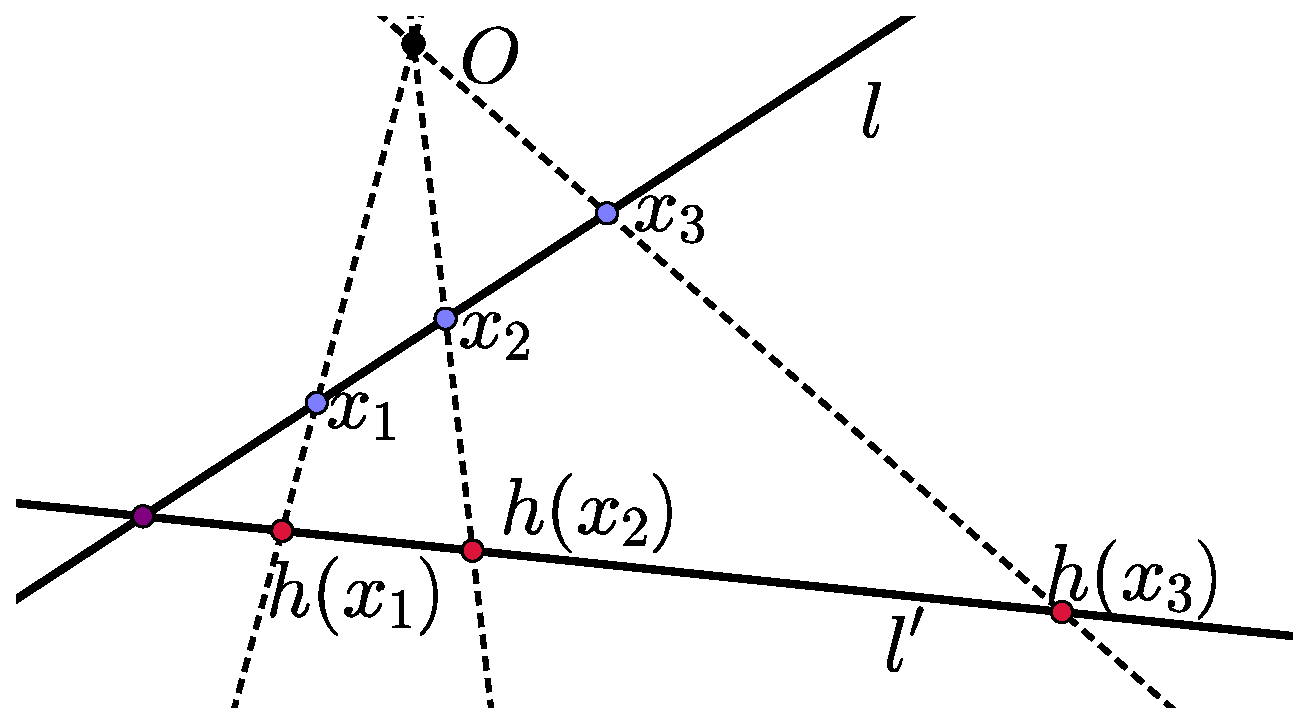
\includegraphics[scale=.3]{Graficos/perspectividad.eps}
\end{center}

Así pues, como las homografías conservan la razón doble, calcular la razón doble de los puntos alineados $A,B,C,D$ será equivalente a calcular la razón doble de sus imágenes por $h$. Es decir:
\[\{A,B;C,D\}=\{h(A),h(B);h(C),h(D)\}\]
La utilidad de esto se ve muy claramente cuando se proyecta sobre los ejes coordenados, tal y como muestra el siguiente ejemplo.
\begin{exa}[Proyección sobre los Ejes]\label{C5:ej_proy_sobre_ejes}
	Sean los puntos $A,B,C,D$ del ejemplo \ref{C5_exa_puntosAlineados}. Tomemos el punto $O=(1:0:0)\not\in AB$ y la recta $r:=AB$. Tomamos asimismo la recta $r'$ definida por la ecuación implícita $x=0$ (eje de coordenadas de $\proy^2$).
	
	Consideramos la proyección $\pi$ del ejemplo \ref{C4_exa_fabricaHomografias}, que a cada punto $x$ de la recta $r$ le asocia el punto intersección de la recta $Ox$ con la recta $r'$. Hallando esta intersección de forma genérica (como aprendimos en \ref{C3_interseccionRectas}) obtenemos la siguiente fórmula explícita para $\pi$:
	\[\begin{array}{c}
	r\setminus\{O\}\stackrel{\pi}{\to} r'\\
	P=(a:b:c)\mapsto\class{(a,b,c)-a(1,0,0)}=(0:b:c)
	\end{array}\]
	De esta forma, como las homografías preservan la razón doble, tenemos que:
	\[\{A,B;C,D\}=\{\pi(A),\pi(B);\pi(C),\pi(D)\}=\{(0:0:-1),(0:1:0);(0:1:-2),(0:1:1)\}\]
	Si ahora consideramos la homografía $\pi'$ que identifica canónicamente a la recta $r'$ con $\proy^1$, dada por la proyección
	\[\begin{array}{c}
	r'\stackrel{\pi'}{\to}\proy^1\\
	x=(0:b:c)\mapsto(b:c)
	\end{array}\]
	de nuevo, como las homografías preservan la razón doble obtenemos:
	\[\{A,B;C,D\}=\{(0:-1),(1:0);(1:-2),(1:1)\}\]
	Y esto ya lo sabemos calcular. Nótese que nos debería dar el mismo resultado que el ejemplo \ref{C5_exa_puntosAlineados}. En efecto:
	\[\{A,B;C,D\}=\left\{0,\infty;-\frac{1}{2},1\right\}=\frac{\frac{1}{2}}{\infty+\frac{1}{2}}:\frac{-1}{\infty-1}=-\frac{1}{2}\]
	Para que la proyección a aplicar sea una homografía es fundamental que el centro de proyección $O$ no pertenezca a la recta en la que los cuatro puntos están alineados.
\end{exa}

La aplicación de uno u otro método (o una combinación de ambos) hace que los cálculos sean mucho más rápidos y sencillos.
\subsection{Razón Doble y Dualidad}
Un paso más en lo que concierne a estas generalizaciones es trasladar todos estos conceptos al espacio dual. Si lo hacemos (estando en $\proy^2$) obtendremos el concepto de razón doble de cuatro rectas concurrentes.

Recordemos que cuatro rectas concurrentes son cuatro rectas que se cortan en un mismo punto. Por tanto, forman un haz de rectas en $\proy^2$ con base el punto de corte. Dado que, como se vio en capítulos anteriores, un haz de rectas en un $\proy^1$ en el espacio proyectivo dual y sabemos calcular la razón doble para puntos de $\proy^1$, si tomamos las rectas como puntos del dual, podremos calcular su razón doble.

Así pues, definimos la razón doble de cuatro rectas concurrentes como la razón doble de los puntos que se corresponden las $4$ rectas en el dual.

Dadas $4$ rectas proyectivas $r_1,r_2,r_3,r_4$ estando cada una de ellas definida por cierta ecuación implícita, se tiene que:
\[r_i:a_ix+b_iy+c_iz=0\]
Sabemos que el punto proyectivo del dual asociado a esa recta es el punto $(a_i:b_i:c_i)$.

De esta forma se tiene que:
\[\{r_1,r_2;r_3,r_4\}=\{(a_1:b_1:c_1),(a_2:b_2:c_2);(a_3:b_3:c_3),(a_4:b_4:c_4)\}\]
Pongamos un ejemplo con rectas concretas para verlo más claro.
\begin{exa}[Razón Doble de Cuatro Rectas Concurrentes]
	Dadas las rectas:
	\[\begin{array}{c}
	r_1:x-y=0\\
	r_2:x+z=0\\
	r_3:2x-y+z=0\\
	r_4:y+z=0
	\end{array}\]
	La razón doble de las mismas, dualizando y proyectando, como vimos en el ejemplo~\ref{C5:ej_proy_sobre_ejes}, queda
	\[\{(1:-1:0),(1:0:1);(2:-1:1),(0:1:1)\}=\{\infty, 0; -1,1\}=-1\]
	Hecho esto, podemos extender el concepto de cuaterna armónica a cuaterca armónica formada por cuatro rectas concurrentes.
\end{exa}
\subsubsection{Método de los Haces de Rectas}
Otra forma de calcular la razón doble de cuatro rectas concurrentes es recurrir a los haces de rectas. Expliquemos esto. Dadas cuatro rectas $r_1,r_2,r_3,r_4$ que se cortan en un mismo punto $O$, consideremos el haz de rectas de base $O$, al que denotaremos por $\haz_O$. Sea otra recta $l$ que no pertenece al haz y consideremos la aplicación proyectiva
\[\begin{array}{cccc}
h:&\haz_O&\rightarrow & l\\
& r&\rightarrow & r\cap l
\end{array}\]

\begin{center}
	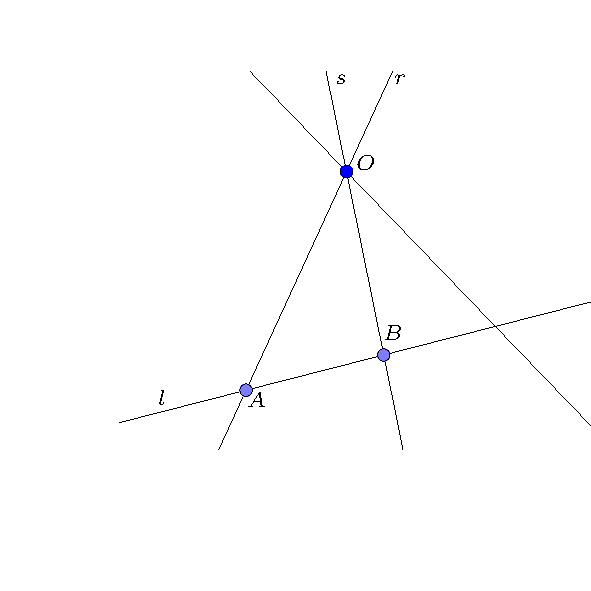
\includegraphics[scale=.8]{Graficos/RazonDoble/rectas_dual}
\end{center}
Si demostramos que $h$ es una homografía, entonces
\begin{equation}
 \{r_1,r_2;r_3,r_4\}=\{h(r_1),h(r_2);h(r_3),h(r_4)\}=\{r_1\cap l,r_2\cap l;r_3\cap l,r_4\cap l\}
\end{equation}
Para ello, veamos cual es la imagen de una recta arbitraria del haz. Es necesario, entonces, parametrizar el haz y tomar una referencia.

Sean $r,s\in\haz_O$ dos rectas distintas del haz y consideremos a referencia $\mf{R}=\{O,h(r),h(s);e\}$ de $\proy^2$. Denotando $h(r)=A$ y $h(s)=B$, la referencia queda $\mf{R}=\{O,A,B;e\}$. Como $h(r)=r\cap l $ y $h(s)=s\cap l$, se tiene que
\[\begin{array}{c}
r_1=lA:z=0\\
s=lB:y=0\\
l=AB:x=0
\end{array}\]
Tomamos entonces como referencia del haz $\mf{\overline{R}}=\{s=[y=0],r=[z=0];[y+z=0]\}$. Así, una recta arbitraria $m\in\haz_O$ puede escribirse como $m:y+\theta z=0$ para cierto $\theta\in\overline{\K}$. De esta forma, $h(m)=m\cap l=(0:-\theta:1)$. Por tanto, la aplicación definida se describe a través de la ecuación $h(\theta)=\theta'=-\theta$ que no es más que una transformación de Möbius. Por tanto, $h$ es una homografía.

Una observación importante es la siguiente.
\begin{lem}
	Cuatro puntos del plano proyectivo $P_1,P_2,P_3,P_4$ forman una cuaterna armónica entonces las rectas $DP_1,DP_2,DP_3,DP_4$ forman una cuaterna armónica de rectas en el dual, donde $D$ es un punto arbitrario.
\end{lem}
\begin{proof}
	Basta fijarse en la construcción del cuadrilátero completo. Tomaremos los mismos nombres de los puntos de corte para que la explicación resulte más sencilla.
	
	Si $P_1,P_2,P_3,P_4$ forman una cuaterna armónica entonces podremos construir un cuadrilátero completo, donde los puntos $D,F$ serán arbitrarios. Si consideramos las rectas $DP_1,DP_2,DP_3,DP_4$, pertenecientes al haz $\haz_D$ y tomamos como recta $l$ la recta $P_1P_2$, se tiene que
	\[\{DP_1,DP_2;DP_3,DP_4\}=\{P_1,P_2;P_3,P_4\}=-1\]
\end{proof}
Esto nos muestra que, cuando tengamos un cuadrilátero completo, no solo formarán una cuaterna armónica los puntos $P_1,P_2,P_3,P_4$, sino también las rectas antes mencionadas.

Por último, veamos un ejemplo.
\begin{exa}
	Consideremos las rectas concurrentes del ejercicio anterior, es decir
	\[\begin{array}{c}
	r_1:x-y=0\\
	r_2:x+z=0\\
	r_3:2x-y+z=0\\
	r_4:y+z=0
	\end{array}\]
	y tomemos como recta $l:x=0$. La razón doble de las cuatro rectas concurrentes es
	 \begin{multline*}
	 	\{r_1,r_2;r_3,r_4\}=\{r_1\cap l,r_2\cap l;r_3\cap l,r_4\cap l\}0\\
	 	=\{(0:0:1),(0:1:0);(0:1:1),(0:1:-1)\}=\{\infty, 0; -1,1\}=-1
	 \end{multline*}
\end{exa}
Este método para calcular la razón doble puede extenderse a un haz de hiperplanos. Análogamente al caso de rectas, si se tienen $\sigma_1,\sigma_2,\sigma_3,\sigma_4$ hiperplanos de $\proy^n$ distintos pertenecientes a un haz de hiperplanos $\haz_\pi$ y sea $r\subset\proy^n$ una recta tal que $r\cap\pi=\emptyset$, entonces
\begin{equation}
	\{\sigma_1,\sigma_2;\sigma_3,\sigma_4\}=\{\sigma_1\cap r,\sigma_2\cap r;\sigma_3\cap r,\sigma_4\cap r\}
\end{equation} 